%%%%%%%%%%%%%%%%%%%%%%%%%%%%%%%%%%%%%%%%%%%%%%%%%%%%%%%%%%%%%%%%%%%%%%%%%%
%%%%%                         CHAPITRE 1                            %%%%%%
%%%%%%%%%%%%%%%%%%%%%%%%%%%%%%%%%%%%%%%%%%%%%%%%%%%%%%%%%%%%%%%%%%%%%%%%%%

\lhead[\fancyplain{}{\leftmark}]%Pour les pages paires \bfseries
      {\fancyplain{}{}} %Pour les pages impaires
\chead[\fancyplain{}{}]%
      {\fancyplain{}{}}
\rhead[\fancyplain{}{}]%Pour les pages paires 
      {\fancyplain{}{\rightmark}}%Pour les pages impaires \bfseries
\lfoot[\fancyplain{}{}]%
      {\fancyplain{}{}}
\cfoot[\fancyplain{}{\thepage}]%\bfseries
      {\fancyplain{}{\thepage}} %\bfseries
\rfoot[\fancyplain{}{}]%
     {\fancyplain{}{\scriptsize}}


%%%%%%%%%%%%%%%%%%%%%%%%%%%%%%%%%%%%%%%%%%%%%%%%%%%%%%%%%%%%%%%%%%%%%%%%%%
%%%%%                      Start part here                          %%%%%%
%%%%%%%%%%%%%%%%%%%%%%%%%%%%%%%%%%%%%%%%%%%%%%%%%%%%%%%%%%%%%%%%%%%%%%%%%%
\renewcommand\chapterheadstartvskip{\vspace*{-2\baselineskip}}
\chapter{Mise en contexte de l'étude}
\label{ch/biblio}

%==============================================================================	Résumé du chapitre

\begin{center}
\rule{0.8\linewidth}{.5pt}
\begin{minipage}{0.8\linewidth}
\smallskip

\textit{Le contexte de la transition à la turbulence est posé dans ce chapitre. Dans un premier temps, la notion du nombre de Reynolds critique et les différents chemins menant à la turbulence sont introduits. La transition à la turbulence se fait de manière passive via des rugosités distribuées en quinconce dans la thèse. La topologie et la structure des écoulements rugueux sont donc présentées dans un second temps. L'accent est ensuite mis sur la transition de type bypass, une transition se caractérisant par une échelle de temps courte. Les objectifs de la thèse sont élucidés à la fin.}

%\smallskip
\end{minipage}
\smallskip
\rule{0.8\linewidth}{.5pt}
\end{center}

\clearpage
\setbeforeminitoc
$~$
\vfill
\minitoc
\vfill
\newpage
\resetafterminitoc
%%%%%%%%%%%%%%%%%%%%%%%%%%%%%%%%%%%%%%%%%%%%%%%%%%%%%%%%%%%%%%

\begin{figure}[!hbtp]
    \centering
    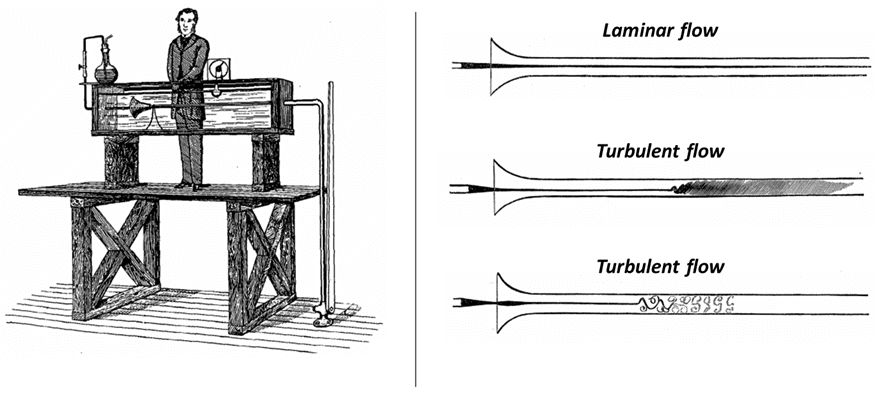
\includegraphics[width=0.925\linewidth]{Chap1/Pictures/Reynolds_Experiment.png}
    \caption{Schéma illustrant les expériences de \citet{Reynolds1883} dans une conduite cylindrique rectiligne qui ont mis en évidence les régimes laminaire et turbulent.}
    \label{fig/reynolds_experiments}
\end{figure}

D'un point de vue historique, la transition à la turbulence a été analysée pour la première fois par \citet{Reynolds1883} à travers des expériences reconnues pour être minutieusement menées malgré la limitation des moyens évidents de l'époque (\cref{fig/reynolds_experiments}). Reynolds a mis en évidence deux régimes d'écoulement en faisant varier le débit, et donc la vitesse dans la conduite : le régime laminaire et le régime turbulent. L'écoulement était laminaire pour de faibles vitesses et le colorant injecté ne se mélangeait pas. La turbulence apparaissait en augmentant la vitesse et le colorant commençait à se mélanger jusqu'à devenir diffus dans toute la conduite. Les deux régimes d'écoulement se caractérisent par un nombre adimensionnel appelé le nombre de Reynolds. Il est le rapport entre les forces inertielles et les forces visqueuses du fluide :

\begin{equation*}
    Re = \frac{U D}{\nu}
\end{equation*}

avec $U$ la vitesse dans la conduite, $D$ le diamètre de la conduite et $\nu$ la viscosité cinématique du fluide. Les forces visqueuses prédominent lorsque l'écoulement est laminaire alors que pour un écoulement turbulent, les forces inertielles dominent. Initialement, la conduite cylindrique est laminaire et l'énergie injectée dans celle-ci à travers le débit se caractérise par l'énergie $\epsilon_{i}^{0}$ (\cite{Bourgoin_Lecture}). Cette dernière peut être dissipée par $\left( \epsilon_{d}^{0} \right)^{max}=\nu^{3}/D^{4}$ qui dépend du diamètre de la conduite. Si l'énergie injectée peut se dissiper à l'échelle $D$ ($\epsilon_{i}^{0}<\left( \epsilon_{d}^{0} \right)^{max}$), alors l'écoulement reste laminaire par équilibre énergétique. En revanche, si $\epsilon_{i}^{0}>\left( \epsilon_{d}^{0} \right)^{max}$, l'énergie injectée dans la conduite ne peut plus être dissipée par la dissipation à sa propre échelle $D$. Il y a donc un transfert d'énergie vers de nouvelles échelles de taille $k<D$ et l'écoulement transite à la turbulence. C'est la cascade de \citet{richardson1922} (\cref{fig/richardson_cascade}). L'énergie qui n'a pas pu être dissipée à l'échelle $D$ devient l'énergie injectée pour la prochaine échelle. En d'autres termes, l'énergie dissipée pour chaque échelle $k$ est $\epsilon_{d}^{k}$ et l'énergie injectée est $\epsilon_{i}^{k}=\epsilon_{i}^{0}-\sum_{j=0}^{k-1} \epsilon_{d}^{j}$. Le transfert d'énergie continu tant qu'à l'échelle $k$, l'équilibre entre l'énergie injectée et l'énergie dissipée n'est pas atteint. L'écoulement a fini de transiter lorsque $\epsilon_{i}^{k}=\epsilon_{d}^{k}$ à l'\foreignquote{french}{échelle de Kolmogorov}, notée $\eta$.

\begin{figure}[!hbtp]
    \centering
    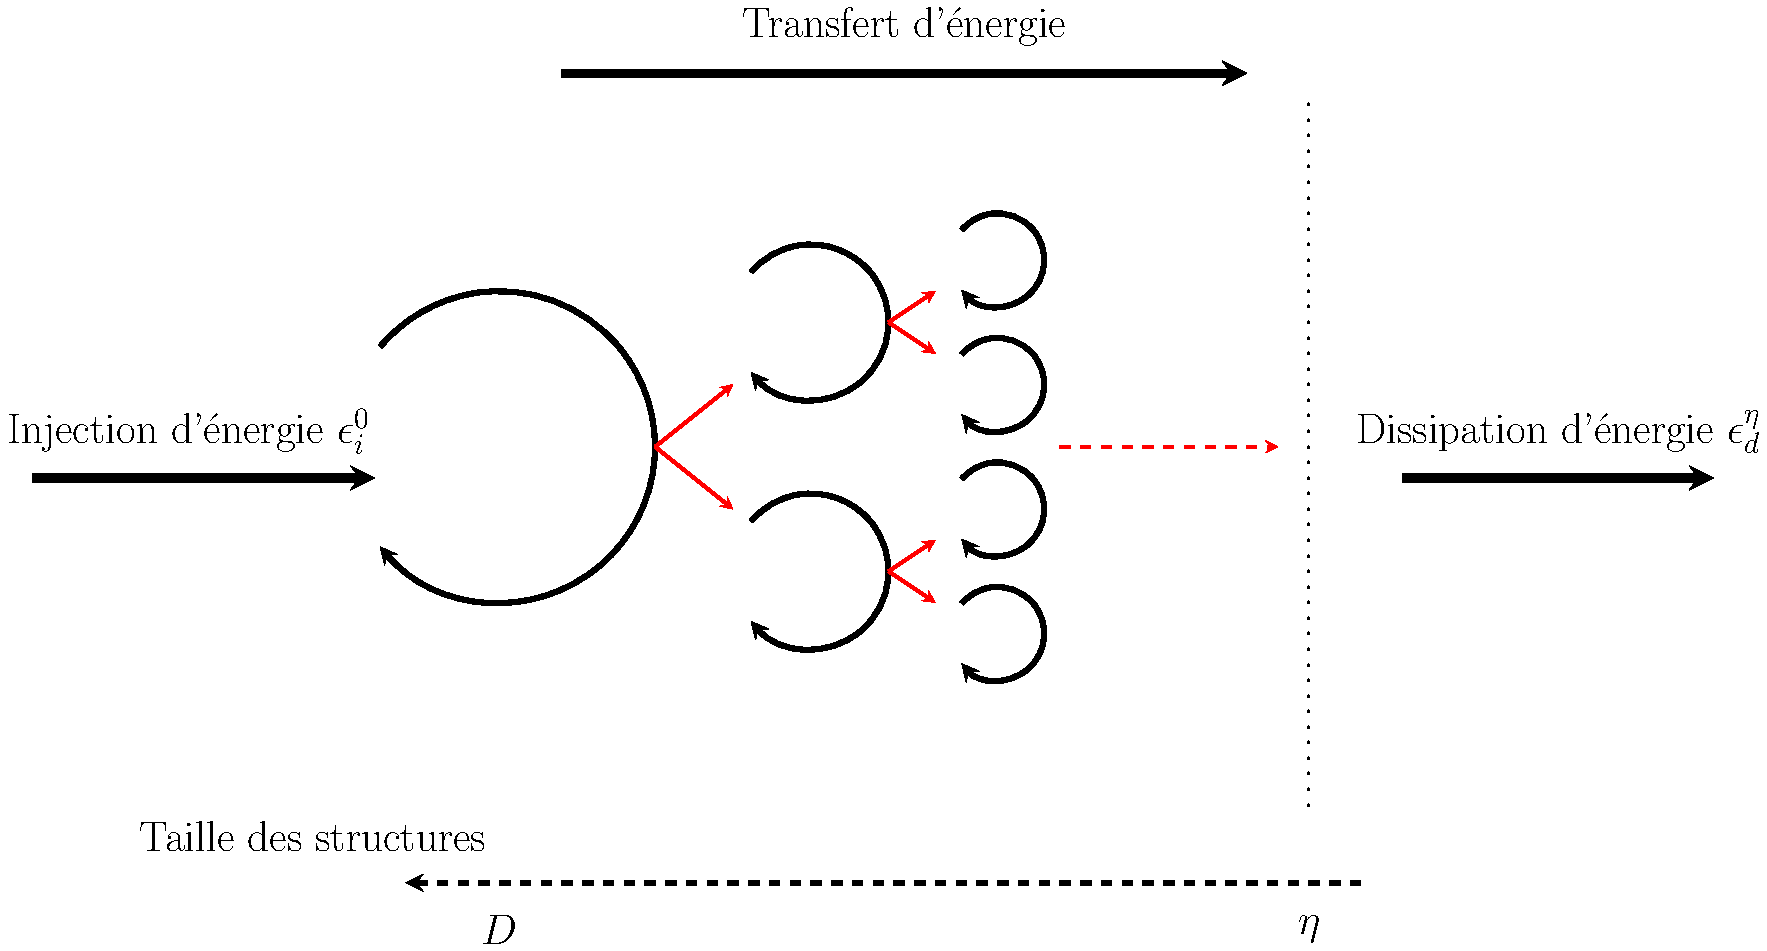
\includegraphics[width=\linewidth]{Chap1/Pictures/richardson_cascade.pdf}
    \caption{Schéma illustrant la cascade d'énergie de \citet{richardson1922}.}
    \label{fig/richardson_cascade}
\end{figure}

\section{Les différents chemins de la turbulence}
\label{sec/path_to_turbulence}

La turbulence se développe lorsque le nombre de Reynolds est très grand devant $1$. Contrôler ou transiter à un écoulement turbulent nécessite de connaître le nombre de Reynolds à partir duquel un écoulement, s’il est perturbé, peut transiter à la turbulence. Il est appelé nombre de Reynolds critique ou sub-critique $Re_{cr}$. Lorsque $Re \approx Re_{cr}$, la turbulence se manifeste comme une multitude de régions turbulentes localisées et entourées d’écoulement laminaire (\cite{Wygnanski1973}). Ce nombre de Reynolds est aussi appelé \foreignquote{french}{point de selle chaotique} dans la littérature (\cite{Eckhardt2007}). Il a été le sujet de plusieurs études et les nombres de Reynolds $Re_{cr}$ suivants sont basés sur la demi-hauteur $H$ d'un canal ou le rayon $R$ d'une conduite cylindrique. \cite{Orszag1971} a trouvé $Re_{cr}=5 772$ par stabilité linéaire en résolvant numériquement l’équation d’Orr-Sommerfeld. \cite{Stuart1960} a trouvé $Re_{cr}=2800$ par stabilité non linéaire. Par la suite, \citet*{Orszag1980} ont mené des simulations numériques directes dans un canal et ont montré que $Re_{cr} \approx 1000$, et qu’à $Re=500$, il était impossible de maintenir la turbulence dans le canal. Leurs simulations numériques directes ont été réalisées dans de petits domaines de calcul dû aux moyens limités de l'époque. Le nombre de Reynolds sous-critique n'est toujours pas clairement identifié de nos jours, car la transition dépend de l'amplitude de la perturbation dans le régime sous-critique. Les études récentes montrent cependant que le nombre $Re_{bcr}$ (basé sur la vitesse débitante $u_{b}$) est $Re_{bcr} \approx 800$ (\cite{Yimprasert2021}).\\

Les écarts observés dans la littérature pour les différents nombres de Reynolds critique s’expliquent par le fait qu’il existe une plage de nombres de Reynolds dans laquelle l’écoulement atteint un état bistable (ou métastable) caractérisé par la coexistence de patchs laminaires et turbulents. \cite{Avila2010} ont réalisé des simulations numériques directes afin d’analyser le temps de vie d’un spot turbulent dans des conditions propices à sa décroissance. Leur relaminarisation était définitive dans les simulations lorsque $Re \leq 860$, alors qu’au-dessus de cette valeur critique, la déstabilisation de l'écoulement causée par la relaminarisation mené à la formation d'un nouveau spot turbulent. Plus récemment, \citet{Sano2016} ont étudié expérimentalement la décroissance de la turbulence. L'écoulement était perturbé avec une grille à l'entrée d'un canal, ce qui engendrait la création de spots turbulents. L'intensité turbulente pouvait donc être analysée dans des sections $y-z$ à différentes positions longitudinales dans le canal. Elle restait à peu près constante dans le canal jusqu'à $Re \approx 850$ et décroissait avec la position longitudinale lorsque $Re \leq 850$, ce qui montrait que l'écoulement se relaminarisait. Les résultats obtenus ont supporté l'hypothèse que le temps de vie d'un spot transitionnel suit une loi super-exponentielle (\cite{Hof2008}, \cite{Avila2010}). Elle dépend du nombre de Reynolds, de la taille du domaine et de la taille du spot (\cite{Goldenfeld2010}, \cite{Avila2023}). Par la suite, \cite{Avila2011} ont continué leur étude via des expériences en conduites. Ils se sont focalisés sur la propagation de la turbulence, notamment la multiplication d'un spot turbulent. Le phénomène menant à la création d’un nouveau spot provient du détachement d’une couche de vorticité suffisamment loin du spot principal. Le temps de multiplication suit également une loi super-exponentielle. L’intersection des lois que suivent les temps de vie et de multiplication permet d’avoir une estimation du $Re_{cr}$ comme montré sur la \cref{fig/Re_cr_Avila_2011}. Ils ont montré que $Re_{cr} \approx 1020$ dans leur cas, ce qui est proche de la valeur obtenue en canal par \cite{Orszag1980}.\\

\begin{figure}[!htbp]
    \centering
    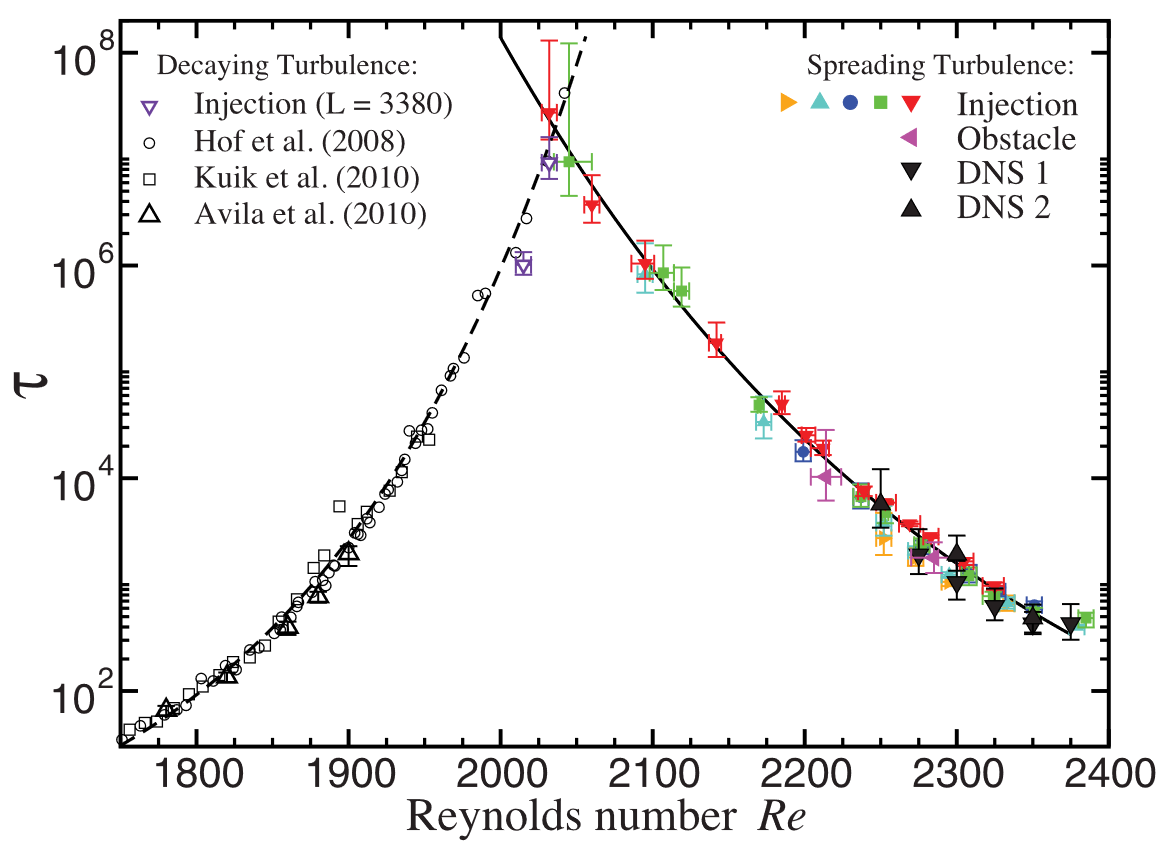
\includegraphics[width=.85\linewidth]{Chap1/Pictures/Re_cr_Avila_2011.png}
    \caption{\centering Temps moyen $\tau$ d'un spot turbulent avant de mourir \refInFig{loi à gauche} ou de se multiplier \refInFig{loi à droite}. L'intersection des deux lois donne $Re_{cr}$. Ce graphique est tiré de \cite{Avila2011}. $Re=UD/\nu$ dans leur étude.}
    \label{fig/Re_cr_Avila_2011}
\end{figure}

\clearpage
Cette thèse a pour but de déclencher la transition d’un écoulement laminaire à un écoulement turbulent. La transition nécessite la perturbation de l’écoulement initial de manière générale. La perturbation peut ensuite emprunter plusieurs \foreignquote{french}{chemins} menant ou non à la turbulence, et le lecteur intéressé pourra se référer à \citet*{Morkovin1994}. Les \foreignquote{french}{chemins} sont présentés sur la \cref{fig/Path_to_transition}. L'étape de réceptivité est primordiale pour un écoulement de couche limite. C'est elle qui définit les caractéristiques initiales de l'instabilité dans la couche limite lorsqu'une perturbation est placée en dehors de la couche limite (\cite{Morkovin1969}). L'instabilité est par la suite amplifiée, que ce soit en couche limite ou dans un canal. Les interactions non linéaires et/ou tridimensionnelles mènent à une amplification rapide des perturbations, créant ainsi les instabilités secondaires. Ces dernières se rompent et créent de la turbulence qui se manifeste dans un premier temps sous la forme de spots transitionnels. C'est l'accroissement spatio-temporel, ainsi que la multiplication des spots qui mène à un canal pleinement turbulent, ou une couche limite pleinement turbulente.

\begin{figure}[!htbp]
    \centering
    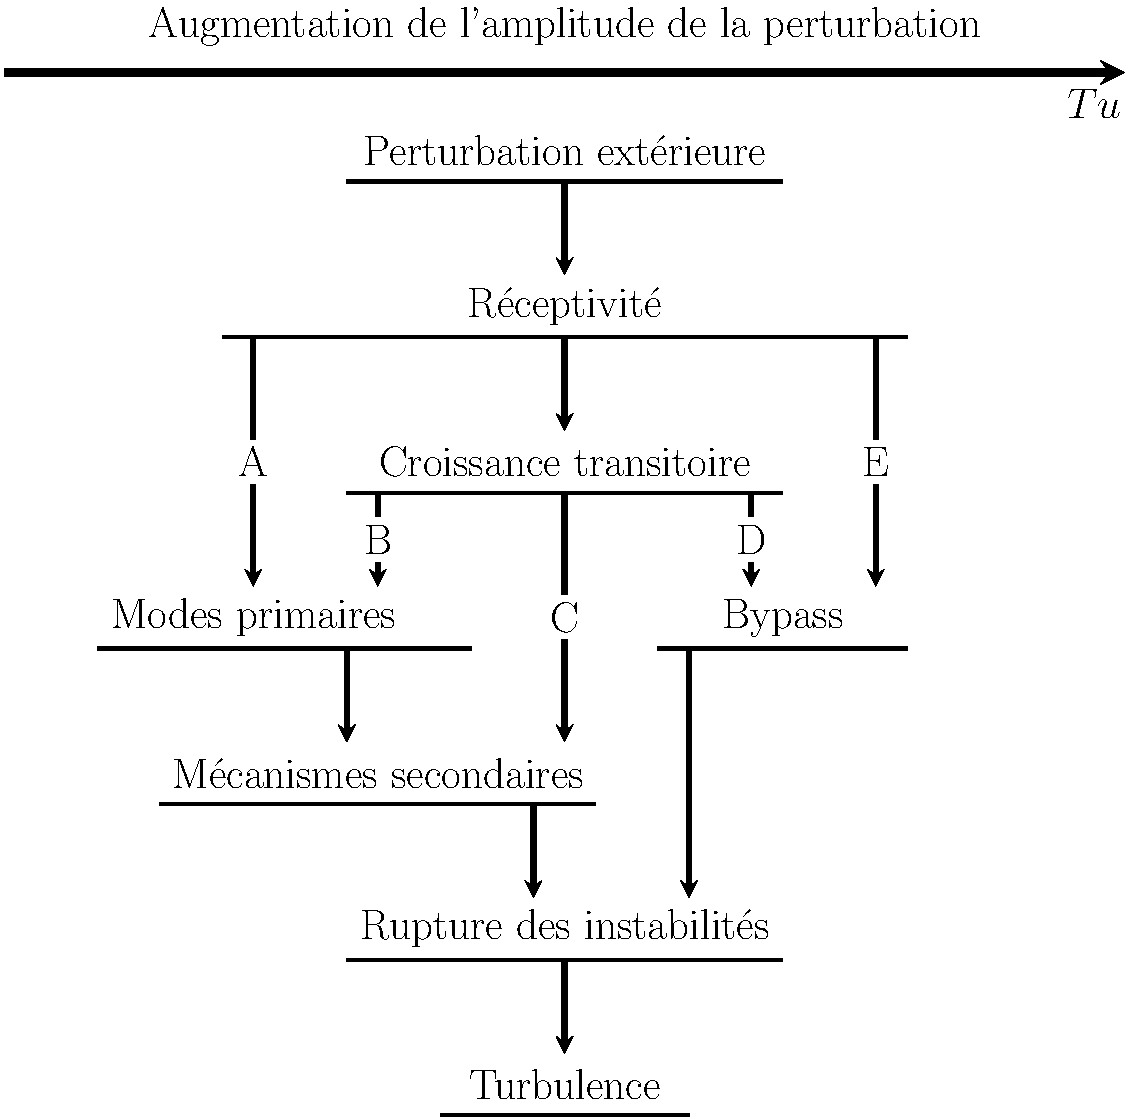
\includegraphics[width=.62\linewidth]{Chap1/Pictures/Path_to_transition.pdf}
    \caption{\centering Les différents chemins menant à la turbulence. Schéma de \cite{Morkovin1994}.}
    \label{fig/Path_to_transition}
\end{figure}

Chaque chemin menant à la turbulence (\cref{fig/Path_to_transition}) a ses spécificités :

\begin{itemize}
    % Chemin A
    \item \textbf{Chemin A :} La perturbation a une très faible amplitude (intensité turbulente $Tu<0.1\%$). L'instabilité engendrée par la perturbation subit une croissance modale exponentielle. Le déclenchement de la transition peut être corrélé à l'amplification modale qui dépend du taux de turbulence (\citet{mack1977}). L'exemple le plus connu est la croissance des ondes de Tollmien-Schlichting. Les instabilités de \foreignquote{french}{crossflow} (pour les couches limites) et de \foreignquote{french}{Görtler} (pour les couches limites sur une surface concave) suivent aussi ce chemin de transition à la turbulence. C'est le chemin qui a été le plus étudié dans la littérature. 

    % Chemin B
    \item \textbf{Chemin B :} La perturbation a une faible amplitude ($0.1\%<Tu<0.7\%$). L'instabilité engendrée a une croissance transitoire lorsque l'amplitude de la perturbation augmente. L'amplitude de la perturbation reste assez faible pour qu'il y ait conjointement une croissance transitoire et une amplification de l'instabilité modale sur le chemin B. Cela a pour conséquence l'intensification de la croissance modale. En couche limite, \citet{Kosorygin1990} avaient montré la coexistence des ondes de Tollmien-Schlichting et des modes de Klebanoff (instabilités associées à la croissance transitoire).

    % Chemin C
    \item \textbf{Chemin C :} La perturbation a une amplitude modérée ($0.7\%<Tu<1\%$). L'amplitude de la perturbation est suffisamment importante pour que la croissance transitoire remplace l'amplification modale.

    % Chemin D
    \item \textbf{Chemin D :} La perturbation a une grande amplitude ($Tu>1\%$). Elle est tellement importante qu'elle donne naissance à plusieurs autres perturbations qui interagissent entre elles, accélérant ainsi la croissance transitoire. L'amplitude de la perturbation permet de \foreignquote{french}{bypasser} l'instabilité modale et les mécanismes secondaires. La croissance transitoire prédomine, ce qui se caractérise par une forte intensification de l'énergie. Cela se traduit par la formation de stries dans l'écoulement. Les perturbations empruntant ce chemin ont été étudiées en détail dans la littérature. Le lecteur intéressé pourra se référer à \citet{Andersson1999} et \citet{Luchini2000} pour des cas en couche limite, et à \citet{Henningson1993} pour un cas en écoulement de Poiseuille. Les perturbations optimales ont la forme de paires de tourbillons contrarotatives dans les deux cas.

    % Chemin E
    \item \textbf{Chemin E :} La perturbation a une très grande amplitude ($Tu>>1\%$). L'amplitude est si importante que l'identification de la croissance transitoire n'est plus possible. La notion de transition est alors discutable.\\
\end{itemize}

Un des objectifs de la thèse est de contrôler passivement la transition d'un écoulement dans la région d'entrée d'un canal comme indiqué dans l'introduction. Deux couches limites se développent sur la paroi inférieure et supérieure dans cette région et la vitesse au centre du canal s'accélère (\cite{Durst2005}). Les deux couches se rejoignent dans la partie pleinement développée du canal. Il faut donc déstabiliser la couche limite à l'aide d'une perturbation extérieure, comme expliqué plus haut. Il existe deux méthodes pour perturber l'écoulement et transiter à la turbulence : les méthodes actives et passives. Les méthodes actives requièrent de l'énergie pour contrôler la turbulence. C'est le cas par exemple de l'utilisation des ultrasons (\cite{Poncet2021}) ou d'actuateurs pariétaux (\cite{Carlson1982}). Les méthodes passives ne requièrent pas d'énergie. C'est le cas par exemple lorsque des rugosités sont utilisées pour déclencher la transition à la turbulence (\cite{Anika2020} ou \cite{Vadlamani2018}). La transition à la turbulence sera déclenchée par une méthode passive avec des rugosités rectangulaires de grandes tailles pour cette thèse. Il convient donc d'introduire la notion d'écoulement rugueux et de comprendre comment les rugosités impactent l'écoulement.

%%%%%%%%%%%%%%%%%%%%%%%%%%%%%%%%%%%%%%%%%%%%%%%%%%%%%%%%%%%%%%%%%%%%%%%%%%%%%%%%%%%%%%%%%%%%%%%%%%%%%%%%%%%%%%%%%%%%%%%%%%%%%%%%%%%%%%%%%%%%%%%%%%%%%%%%%%%%%%%%%%%%%%%%%%%%%%%%%%%
\clearpage
\section{Écoulements rugueux turbulents}

Le premier à avoir étudié des parois rugueuses a été \cite{Nikuradse1933} en collant des grains de sable de différentes tailles $k_{s}$ dans une conduite circulaire. L'ajout de rugosités sur la paroi a un impact sur la vitesse moyenne $\overline{U}$. En effet, à nombre de Reynolds constants, un décalage s'observe entre le profil $\overline{U}$ de la conduite rugueuse et celui de la conduite lisse (\cref{fig/u_mean_rough}). Il se caractérise à travers la fonction de rugosité $\Delta U^{+}$ :

\begin{equation}
	\overline{U}^{+} = \kappa^{-1} ln(y^{+}) + C - \Delta U^{+}
\end{equation}

avec,

\begin{equation}
	\Delta U^{+} = \kappa^{-1} ln(k_{s}^{+}) + A_{k}
	\label{eq/roughness_function_k}
\end{equation}

où $y$ est la position verticale, $\kappa$ représente la constante de Von Karman, $C$ une constante et $A_{k}$ dépend des rugosités et de leurs distributions. Ici, $(~)^{+}$ représente une quantité en unité de paroi (adimensionnée par $\nu$ et $u_{\tau}$). Cette fonction permet de quantifier l'augmentation du frottement causée par l'ajout des rugosités. Elle se retrouve aussi dans les écoulements de couche limite sur plaque plane rugueuse comme l'a montré \cite{Clauser1954}.

\begin{figure}[!hbtp]
    \centering
    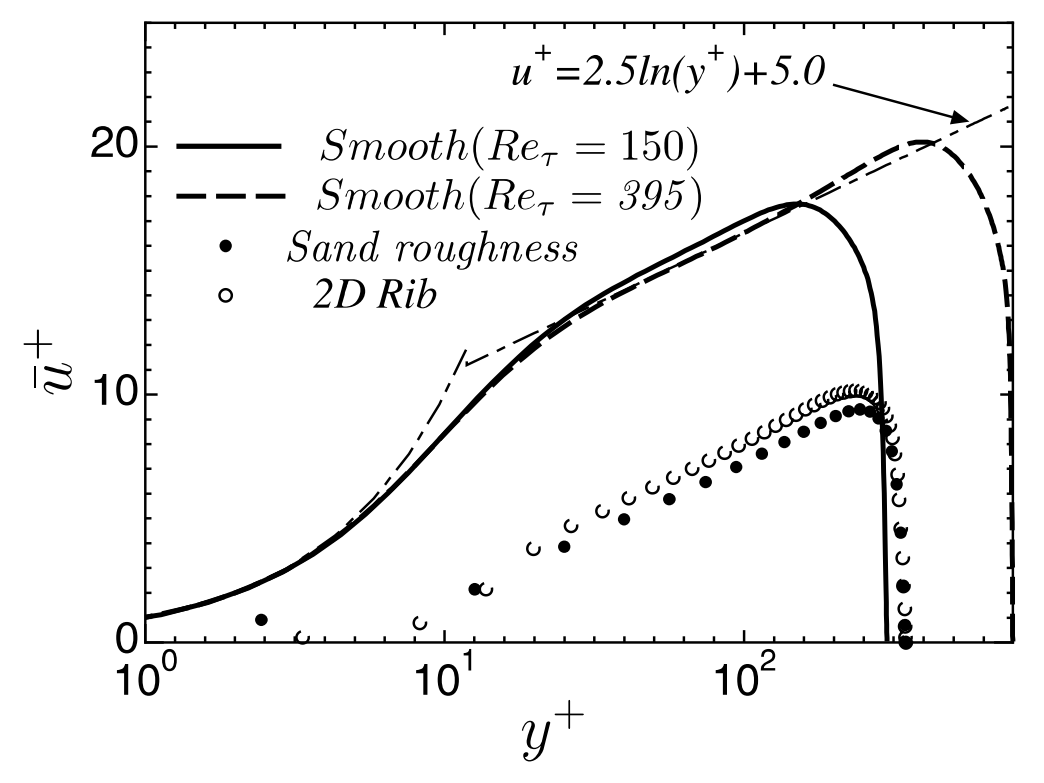
\includegraphics[width=0.65\linewidth]{Chap1/Pictures/Ecoulement_rugueux/U_mean_rough_miyake.png}
    \caption{Profils de vitesse moyenne $\overline{U}^{+}$ obtenus en canal lisse (trait continu et trait en pointillé) et en canal rugueux (symboles) par \cite{Miyake2001}.}
    \label{fig/u_mean_rough}
\end{figure}

L'écoulement se classe en deux types suivant la géométrie utilisée : type $k$ et type $D$ (ou $H$) (\cite{Perry1969}). La différenciation permet de caractériser l'impact des rugosités sur l'écoulement comme expliqué par \cite{Leonardi2007} (\cref{fig/roughness_type}).\\

\begin{figure}[!hbtp]
    \centering
    \captionsetup[subfigure]{justification=centering}
    \begin{subfigure}[b]{\textwidth}
      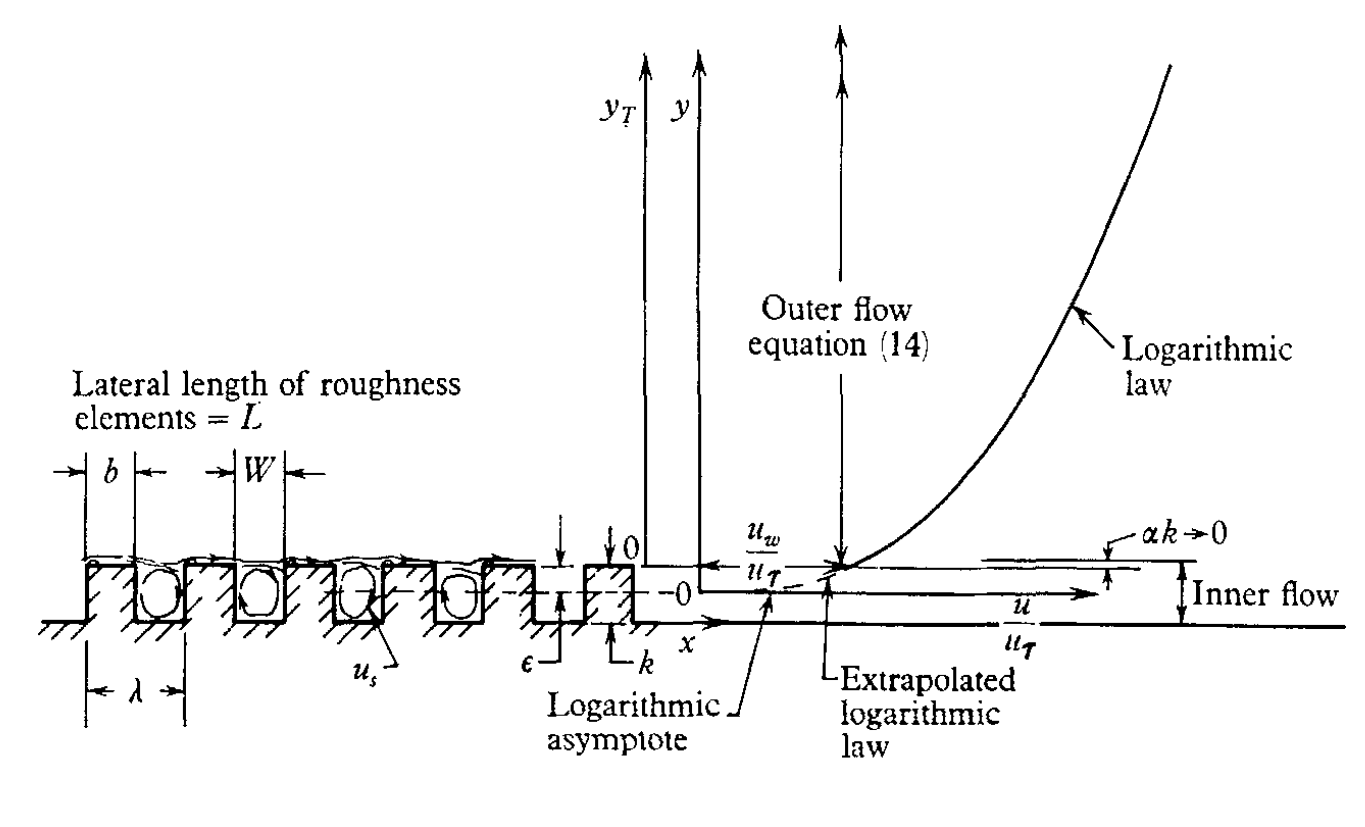
\includegraphics[width=\linewidth]{Chap1/Pictures/Ecoulement_rugueux/d_type_roughness_Perry.png}
      \caption{Rugosité de type $D$ (ou $H$)}
    \end{subfigure}%
    \hspace{1em}
    \begin{subfigure}[b]{\textwidth}
      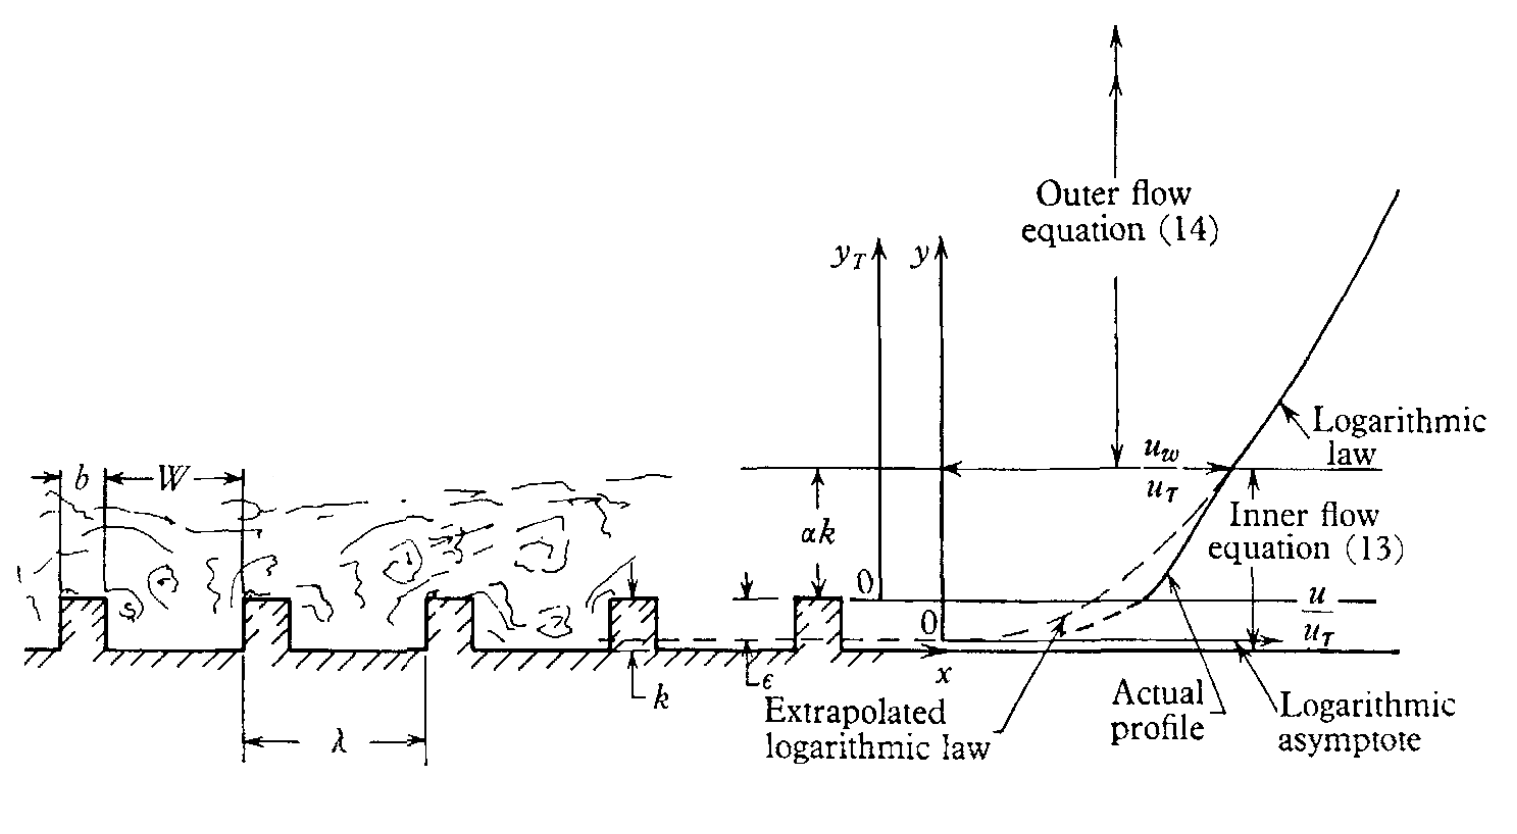
\includegraphics[width=\linewidth]{Chap1/Pictures/Ecoulement_rugueux/k_type_roughness_Perry.png}
      \caption{Rugosité de type $k$}
    \end{subfigure}
    \caption{Schéma montrant l'impact des rugosités de type $D$ (ou $H$) et de type $k$ sur l'écoulement et le profil moyen de vitesse correspondant. Schéma tiré de \cite{Perry1969}.}
    \label{fig/roughness_type}
\end{figure}

\clearpage
Les rugosités génèrent des structures tourbillonnaires de taille $k$ qui se diffusent dans l'écoulement pour les rugosités de type $k$. La fonction de rugosité dépend alors de la taille des rugosités et s'écrit de la même manière que dans l'\cref{eq/roughness_function_k}. Il y a des tourbillons stables entre les rugosités pour les rugosités de type $D$ (ou $H$) et les phénomènes d'éjection de fluide sont moins importants. Dans ce cas, la fonction de rugosité dépend du diamètre $D$ de la conduite ou de la hauteur $H$ du canal et s'écrit :

\begin{equation}
	\Delta U^{+} = \kappa^{-1} ln(D^{+}) + A_{D}
	\label{eq/roughness_function_D}
\end{equation}

où $A_{D}$ est une constante qui dépend des rugosités et de leur distribution.\\

Il n'existe pas de consensus pour déterminer a priori si l'écoulement sera de type $k$ ou $D$ avec la configuration et les rugosités utilisées. \cite{Leonardi2007} ont essayé de caractériser les types de rugosités avec des simulations SND et des rugosités rectangulaires et triangulaires couvrant la largeur du canal. Ils ont notamment montré que les rugosités de type $D$ produisaient une traînée visqueuse nettement supérieure à la traînée de forme.\\

%%%%%%%%%%%%%%%%%%%%%%%%%%%%%%%%%%
La fonction de rugosités $\Delta U^{+}$ a longtemps été considéré comme suffisante pour caractériser une forme de rugosité et une configuration. Il est compliqué d'obtenir une prédiction exacte en proche rugosité d'un point de vue expérimental (\cite{Bakken2005}). Cela requiert de grands moyens de calcul d'un point de vue numérique, car il faut tester chaque rugosité et chaque configuration qui sont uniques. De ce fait, au lieu de caractériser la résistance hydraulique ou le coefficient de friction de chaque configuration, il est plus intéressant d'établir la taille de grain de sable équivalent $k_{s}$ (en référence au travail de \cite{Nikuradse1933}). Les diagrammes de \cite{Moody1944} valable en conduite ou en canal, et ceux de \cite{Prandtl1955} ou \cite{Granville1958} valable en couche limite, peuvent ensuite être utilisés pour prédire le coefficient de friction de la configuration.\\

\cite{Chung2015} ont conduit des simulations numériques directes afin de quantifier l'impact de la dimension transversale du domaine sur la fonction de rugosités. Leur idée était de s'inspirer du travail de \cite{Jimenez1991} et \cite{Flores2010} sur les tailles minimales en canaux lisses et d'étendre leurs conclusions aux parois rugueuses. Ils ont développé une méthode numérique rapide et efficace pour caractériser la fonction de rugosités pour une configuration donnée. Elle permet notamment d'économiser des heures de calcul.\\   

%%%%%%%%%%%%%%%%%%%%%%%%%%%%%%%%%%
Un autre pionnier dans le domaine des écoulements rugueux est \cite{Townsend1976} avec l'hypothèse de similarité de paroi stipulant l'existence d'une sous-couche rugueuse s'étendant jusqu'à $y^{*} \sim 5 k^{*}$. Au-delà, les rugosités n'ont plus d'impact sur l'écoulement (\cref{fig/roughness_sublayer}). Par conséquent, l'écoulement obtenu avec une paroi rugueuse est équivalent à celui obtenu avec une paroi lisse à haut $Re$ en dehors de la sous-couche rugueuse.\\

\begin{figure}[!hbtp]
    \centering
    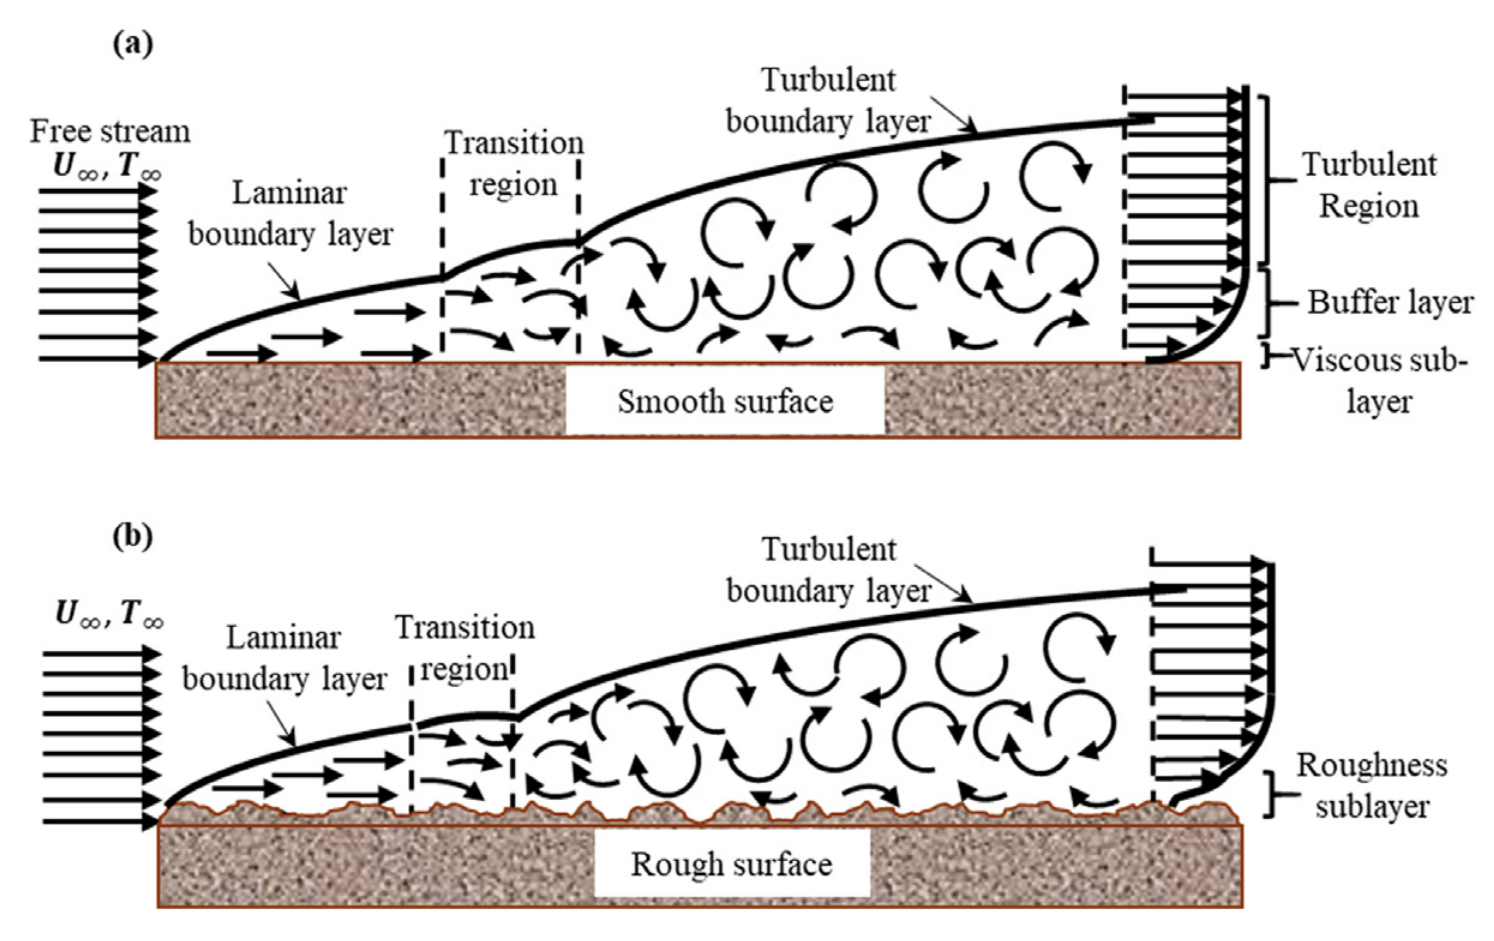
\includegraphics[width=\linewidth]{Chap1/Pictures/Ecoulement_rugueux/roughness_sublayer_Kadivar.png}
    \caption{Représentation schématique de l'impact des rugosités sur le profil de vitesse moyenne en couche limite. Les rugosités ont un impact dans la sous-couche rugueuse. Schéma tiré de \cite{Kadivar2021}.}
    \label{fig/roughness_sublayer}
\end{figure}

\vspace{1.25cm}
La théorie de Townsend a été supportée et renforcée par les résultats expérimentaux de \cite{Perry1969} et \cite{Raupach1991}. Les expériences des premiers ont permis de mettre en évidence l'existence d'écoulement rugueux de type $k$ et $D$ (ou $H$). Les expériences des seconds ont renforcé la théorie de similarité de \cite{Townsend1976} sur une large gamme de rugosités. Ils ont montré que les rugosités interagissaient fortement avec les tourbillons quasi longitudinaux (TQLs), mais que l'interaction entre la sous-couche rugueuse et la couche externe était faible. De ce fait, uniquement la sous-couche rugueuse diffère d'un écoulement obtenu sur parois lisses. Par la suite, \cite{Jimenez2004} a étendu l'hypothèse de similarité de Townsend en spécifiant que pour éliminer les effets des rugosités dans la couche externe, il fallait vérifier la condition $H/k>40$.\\

La théorie de similarité de \cite{Townsend1976} a ensuite été confirmé et infirmé au fil des expériences et des simulations numériques. Si les rugosités sont placées sur les deux parois d'un canal, alors cette hypothèse est vérifiée quelles que soient les rugosités utilisées et leur distribution (\cite{Lee2002}, \cite{Ashrafian2004}, \cite{Bakken2005}, \cite{Krogstad2005}). De plus, il faut nécessairement une configuration de rugosités avec une distribution irrégulière lorsque celles-ci sont placées uniquement sur une seule paroi d'un canal, ou dans une couche limite. L'hypothèse de similarité de Townsend n'est pas vérifiée lorsque les rugosités couvrent la largeur du canal (barres transversales rectangulaires ou triangulaires (\cite{Djenidi1999}, \cite{Krogstad2005}, \cite{Lee2007})) comme expliqué par \cite{Antonia2001}.

%%%%%%%%%%%%%%%%%%%%%%%%%%%%%%%%%%
L'étude expérimentale de \cite{Hanjalic1972} est aussi un travail important pour les écoulements rugueux et a inspiré de nombreuses études. Ils ont fourni de nombreuses statistiques, ainsi que les spectres et les termes de transport de l'énergie cinétique turbulente grâce à leur étude d'un écoulement turbulent dans un canal possédant une paroi lisse et une paroi rugueuse (\cref{fig/asym_roughness_distrib}). Leur étude a été largement utilisée en simulations numériques comme validation (par exemple le groupe de recherche de Sapienza University of Rome (Orlandi et Leonardi)).\\

\begin{figure}[!hbtp]
    \centering
    \captionsetup[subfigure]{justification=centering}
    \begin{subfigure}[b]{\textwidth}
        \centering
        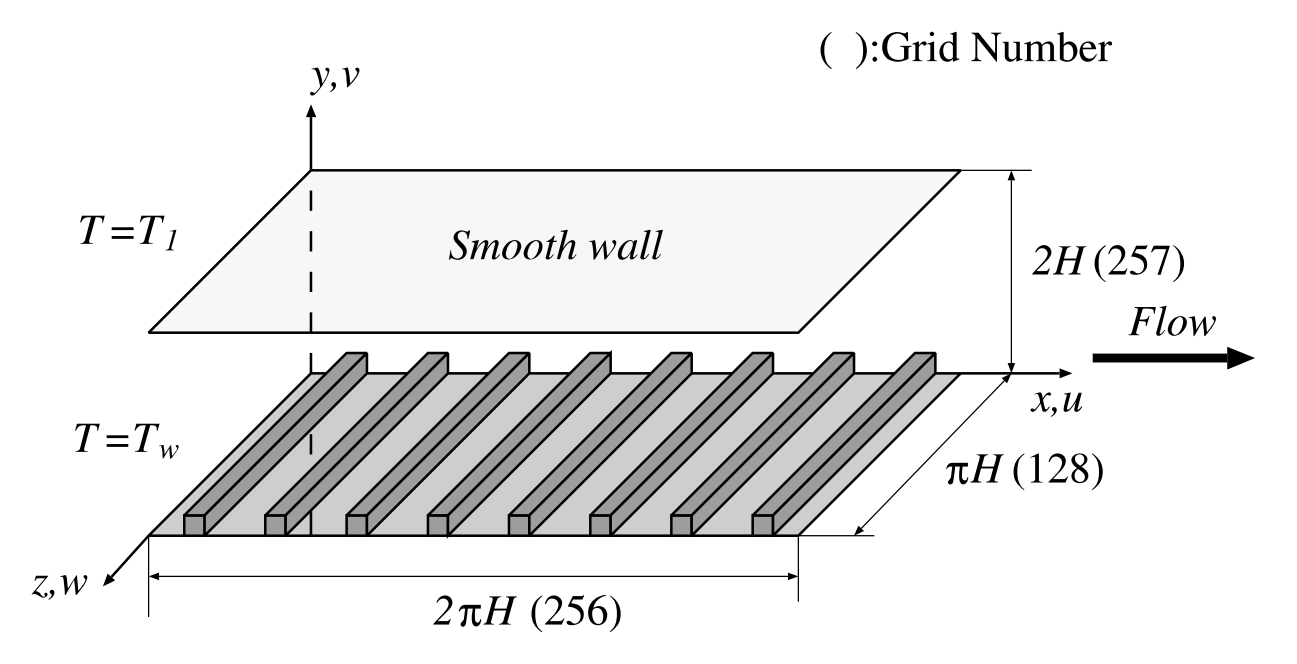
\includegraphics[width=0.7\linewidth]{Chap1/Pictures/Ecoulement_rugueux/asym_rough_miyake.png}
    \end{subfigure}\\
    \begin{subfigure}[b]{\textwidth}
        \centering
        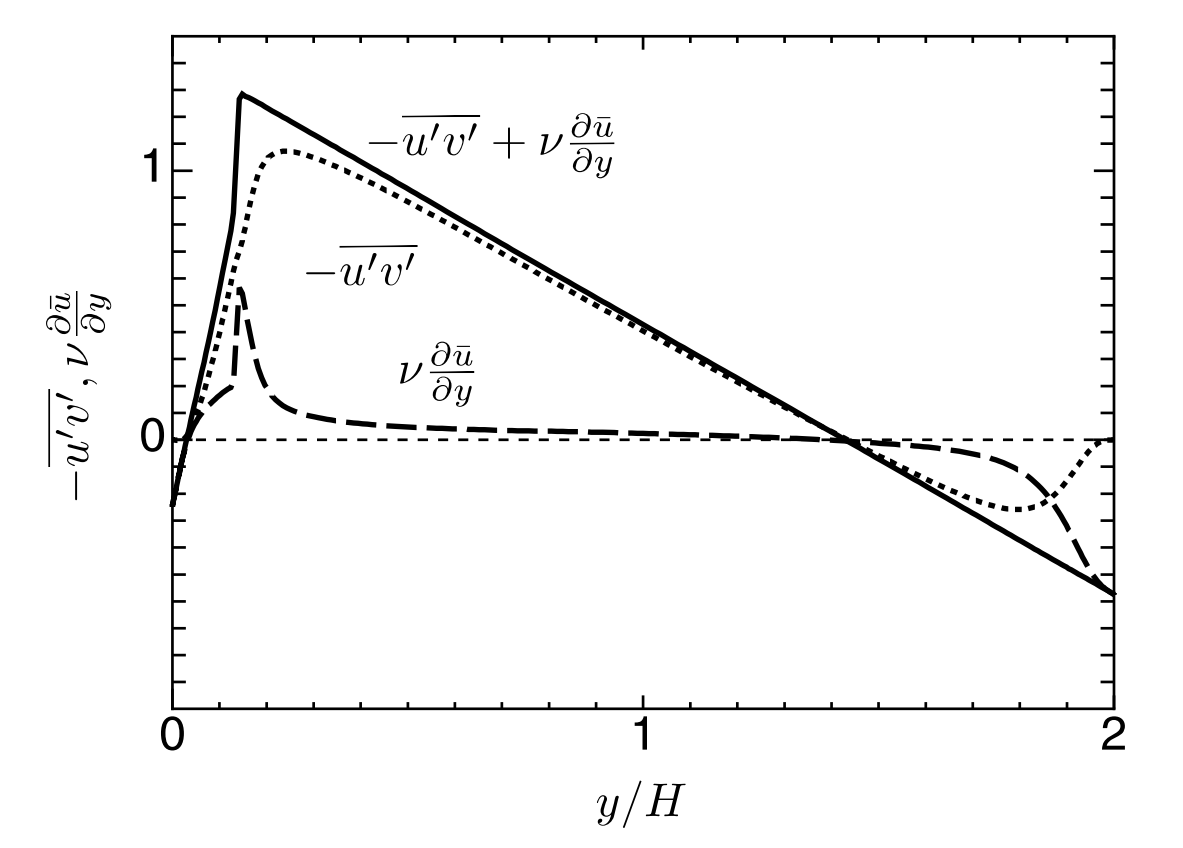
\includegraphics[width=.65\linewidth]{Chap1/Pictures/Ecoulement_rugueux/asym_rough_uv_miyake.png}
    \end{subfigure}
    \caption{Exemple de configuration asymétrique utilisée par \citet{Miyake2001} et la contrainte de Reynolds $-\overline{u'v'}$ associée. Cette dernière est décalée vers la paroi supérieure (lisse).}
    \label{fig/asym_roughness_distrib}
\end{figure}

Les écoulements avec des rugosités placées sur une seule paroi sont différents de ceux avec des rugosités sur les deux parois (\cite{Bakken2005} ou \cite{Krogstad2005}). En effet, il y a un fort effet d'asymétrie qui décale la position du maximum de la vitesse longitudinale et du \foreignquote{french}{$0$} de la contrainte de Reynolds $-\overline{u'v'}$ vers la paroi lisse (\cref{fig/asym_roughness_distrib}). Cependant, les études restent intéressantes pour comprendre l'effet local des rugosités et sont donc citées par la suite.

%%%%%%%%%%%%%%%%%%%%%%%%%%%%%%%%%%%%%%%%%%%%%%%%%%%%%%%%%%%%%%%%%%%%%%%%%%%%%%%%%%%%%%%%%%%%%%%%%%%%%%%%%%%%%%%%%%%%%%%%%%%%%%%%%%%%%%%%%%%%%%%%%%%%%%%%%%%%%%%%%%%%%%%%%%%%%%%%%%%
\clearpage
\section{Synthèse et objectifs de la thèse}

Bien que les spots transitionnels aient été largement étudiés dans la littérature, il n'y a pas d'étude qui analyse le mélange d'un scalaire passif au sein d'un spot transitionnel en écoulement de Poiseuille, ni le potentiel impact de la région d'onde sur le mélange. En effet, les seules études traitant des transferts thermiques au sein des spots ont été réalisées en couche limite. Pour rappel, les spots obtenus en couche limite et en écoulement de Poiseuille sont structurellement différents, il est donc intéressant de revisiter ce cas académique en écoulement de Poiseuille avec l'ajout du transport d'un scalaire passif. C'est l'objet du chapitre 3.\\

Il est important de rappeler que le but de la recherche ci-présente est de déclencher la turbulence ou la pseudo-turbulence dans un écoulement interne initialement laminaire. Le nombre de Reynolds est particulièrement faible et proche de la valeur critique $Re_{c}=1000$ (\cite{Orszag1980} et \cite{Nishioka1985}). La transition nécessite alors des perturbations d'amplitude suffisamment importantes, sinon la pseudo-turbulence induite par la transition bypass se détruit rapidement par viscosité. Une méthode passive a été retenue pour déclencher la transition comme indiqué précédemment. Elle consiste en des rugosités rectangulaires de grandes tailles distribuées en quinconce. La raison de ce choix sera explicitée dans le chapitre 4. En effet, il faut casser la symétrie transversale comme montré par \cite{Anika2020} pour déclencher la transition bypass avec des rugosités rectangulaires de grandes tailles. Cependant, l'impact du décalage entre les rugosités sur la transition n'a pas encore été traité dans la littérature. Une tâche est donc de comprendre comment le décalage des rugosités influe sur l'état (pseudo)turbulent et le mécanisme de transfert convectif induit.\\

Il n’est pas possible d'intervenir dans la partie du canal où l'écoulement est développé pour de nombreuses applications en microfluidique et en particulier pour le refroidissement des lasers à ultra-haute intensité (\hyperref[ch/introduction]{Introduction générale}). Or, tout système impliquant un écoulement en canal quel qu'il soit possède une zone d'entrée hydraulique. Il est dommage de ne pas se servir de cette zone pour modifier les structures de l'écoulement dans la partie développée. L'effet des rugosités distribuées en quinconce dans la zone de développement hydraulique sur la dynamique et les mécanismes de transport scalaire fait l'objet du chapitre 5. La taille du domaine peut être un problème pour réaliser ce type de simulations, car cela augmente le nombre de nœuds de maillage et demande plus de ressources calculatoires. Une nouvelle méthode pour optimiser efficacement le temps de calcul pour des simulations est, entre autres, présentée dans le dernier chapitre.
